\chapter{Analyse af markbilleder} \label{sec:mark}
Denne sektion har til formål at klarlægge udfordringer ved korrespondanceanalysen af markbilleder. Udfordringerne opstilles på baggrund af en analyse af billederne og vil resultere i hypoteser om, hvilke forudsætninger de korrespondanceanalytiske metoder skal besidde for at muliggøre en korrespondanceanalyse.
\section{Flyverute}
Dronens overflyvning foregår ved at dronen får fire punkter, der definere markens placering. Dronen starter derefter i et hjørne og flyver systematisk fra side til side, med samme orientering, for at overflyve hele marken. Dronen starter på en højde af ca. 60 meter og foretager en overflyvning af marken, hvorefter den falder i højde og overflyver marken igen. Processen gentages, ind til dronen er omkring 5-10 meter over marken. I det udvalgte billedsæt er der fire overflyvninger, hvor hver overflyvning foregår på nogenlunde samme højde.
\section{Markbilleder}
I denne opgave er et sæt billeder fra samme overfløjede kornmark anvendt. På billedsættet ses en kornmark, der består af umiddelbare tilfældige kornstrukturer. I enkelte billeder er der traktorspor. Som illustreret i figur <Indsæt billede der viser udsnit af korn>, er kornet af relativ identisk udseende, og det er derfor vanskeligt at differentiere imellem korn områder, da der ikke opstår definerbare mønstre. Ligheden imellem billederne kan derfor besværliggøre korrespondanceanalysen, hvilket gør det interessant at undersøge hvorvidt det er muligt at opnå korrespondancer.
 figur \ref{fig:korn}.
\begin{figure}[H]
    \centering
    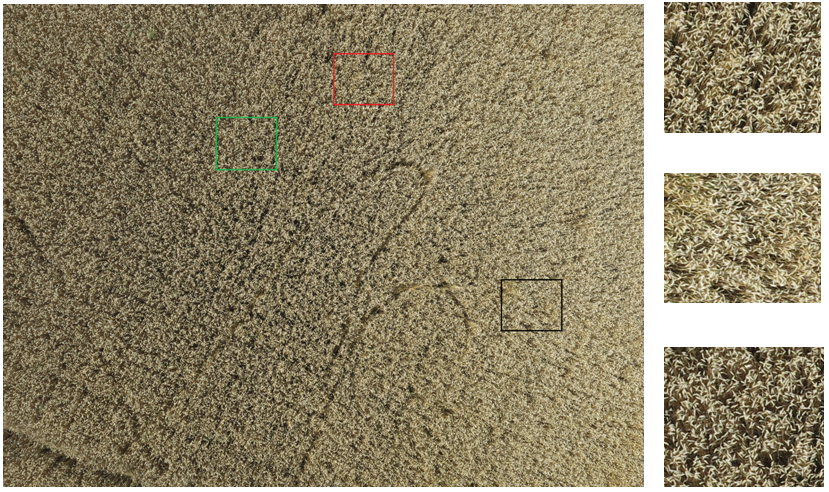
\includegraphics[width=0.65\textwidth]{fig/20.png}
     %\vspace{-1em}
    \begin{center}    
       \caption{\textcolor{gray}{\footnotesize \textit{Markbillederne forstørret ind på enkelte korn.}}}
    \label{fig:korn}
     \end{center}
     \vspace{-2.5em}
  \end{figure} \noindent
Følgende observationer er gjort af markbillederne, samt forhold omkring overflyvningen:
\begin{itemize}
\item{\textbf{Overlap:} Overlappet imellem billederne har en signifikant indflydelse på korrespondanceanalysen. Et stort overlap vil betyde at interessepunkter har større sandsynlighed for at indgå i begge billeder. Derfor, ved mindre overlap, skal der udvælges flere interessepunkter. Det er bekræftet at billederne overlapper hinanden med ca. 70\%\footnote{JOHN}, der forekommer dog store udsving i overlappet, alt efter hvilken højde billederne er taget på. Figur \ref{fig:overlap} viser fire billeder, sat sammen parvist, der er taget ved to forskellige højder, hvor billedernes overlap er markeret med blåt. (a) er taget når dronen er på største højde, billederne er estimeret til at overlappe hinanden med ca. 80 $\%$. (b) er taget ved en lavere højde, billederne overlapper hinanden med ca. 35 $\%$.
\begin{figure}[H]
    \centering
    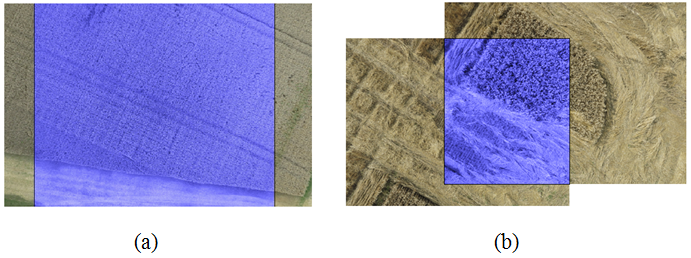
\includegraphics[width=0.65\textwidth]{fig/17.png}
     \vspace{-1em}
    \begin{center}    
       \caption{\textcolor{gray}{\footnotesize \textit{Markbilleder taget fra forskellige højde, det blå område viser billedernes overlap.}}}
    \label{fig:overlap}
     \end{center}
     \vspace{-2.5em}
  \end{figure} \noindent }
\item{\textbf{Rotation:} Der er observeret mindre grad af rotation imellem billederne. Når dronen er nået kanten af marken er det registreret at den i enkelte tilfælde rotere med op til 10-15 $^{\circ}$.
\begin{figure}[H]
    \centering
    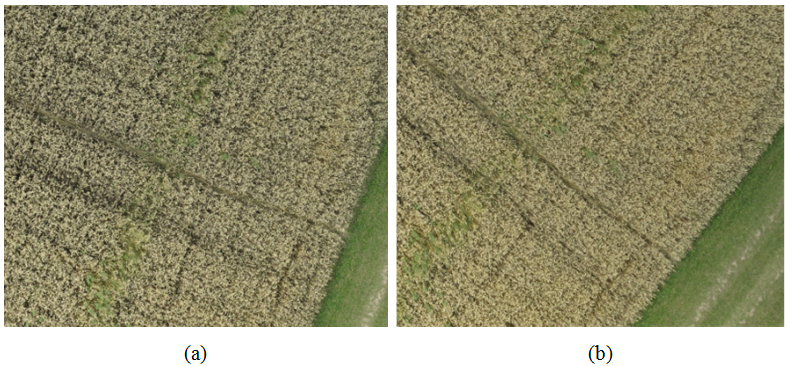
\includegraphics[width=0.65\textwidth]{fig/19.png}
     \vspace{-1em}
    \begin{center} 
       \caption{\textcolor{gray}{\footnotesize \textit{Dronen skal til at ændre retning, hvilket giver rotation i billederne.}}}
    \label{fig:rotation}
     \end{center}
     \vspace{-2.5em}
  \end{figure} \noindent}
\item{\textbf{Okklusion:}
Korn, der stikker direkte op imod kameraet, ses som mørke områder pga. den synlige jord, hvilket vil resultere i et mørkere område direkte under dronen. Forskydes kameraets position, vil det samme område nu ligne korn, da jorden ikke længere kan ses. 
\begin{figure}[H]
    \centering
    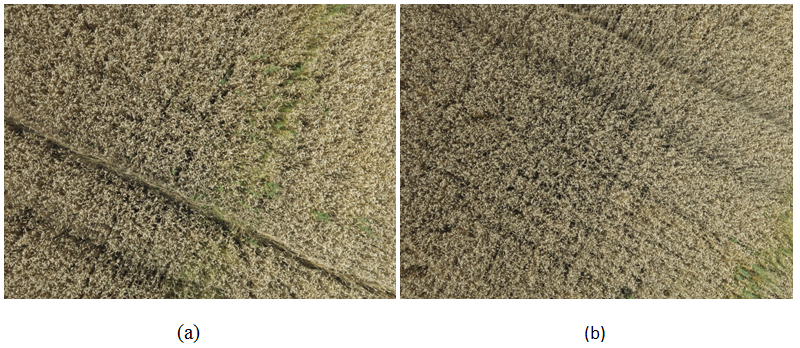
\includegraphics[width=0.65\textwidth]{fig/18.png}
     \vspace{-1em}
    \begin{center}    
       \caption{\textcolor{gray}{\footnotesize \textit{ To forkudte billeder, hvor traktorsporet er okkluderet. }}}
    \label{fig:okklusion}
     \end{center}
     \vspace{-2.5em}
  \end{figure} \noindent
Figur \ref{fig:okklusion} er et eksempel på okklusion af jord, hvor traktor spor optræder direkte under dronen og derefter forskudt. Traktorsporet, der optræder direkte under dronen, er tydelig og man se jorden. For det samme traktorspor, i det forskudte billede, er jorden ikke længere synlig. Det er også værd at bemærke at kornet, direkte under dronen, afgiver mørke områder. Denne okklusion forekommer umiddelbart kun når dronen er på lav højde.}
\item{\textbf{Struktur} }
\end{itemize}
\section{Hypoteser}
Ud fra ovenstående analyse er der opstillet følgende hypoteser om krav til de udvalgte metoder:
\begin{itemize}
\item{ <Det forventes, grundet strukturen af korn, at detektorer som leder efter veldefinerede strukturer, som hjørner, ikke vil have en god effekt på korn, men at blobs vil give bedre resultater.> }
\item{ Det forventes ikke at metoderne behøver være rotationsinvariante, grundet den lille rotation der forekommer imellem billederne. }
\item{Det forventes at metoderne skal være skalainvariante. Bla. for at tilpasse størrelsen af kornet, <men også pga. flere artikler, der strengt understreger nødvendigheden for skalainvarians >.}
\item{ Grundet det til tider lille overlap imellem billeder, forventes det at detektoren skal tilpasses til at finde mange punkter, for at sikre en repeterbar detektion.}
\item{Det forventes ikke at der skal tages højde for problemer ved okklusion, da det kun foregår når dronen flyver lavest. Et overvejet tiltag var ikke at undersøge et område direkte under dronen, men det blev konkluderet at eventuelle nye interessepunkter, der opstår ved okklusion vil sorteres væk som ikke korrespondancer.}
\end{itemize}